\documentclass{article}

\usepackage[final]{neurips_2024}
\makeatletter
\renewcommand{\@noticestring}{}
\makeatother

\usepackage[utf8]{inputenc}
\usepackage[T1]{fontenc}
\usepackage{hyperref}
\usepackage{url}
\usepackage{booktabs}
\usepackage{amsmath}
\usepackage{amssymb}
\usepackage{graphicx}
\usepackage{microtype}
\usepackage{float}

\title{Three-Tier Causal Inference for Anti-VEGF Treatment Comparison in Neovascular Age-Related Macular Degeneration}

\author{%
  Marcus Moen \qquad Sami Barrit \qquad Advaith Veturi \\
  Computational Precision Health \\
  University of California, Berkeley
}

\begin{document}

\maketitle

\begin{abstract}
Aflibercept and ranibizumab are two standard anti-VEGF treatments for neovascular age-related macular degeneration (AMD), a leading cause of irreversible vision loss. A pivotal trial found them equivalent, yet observational comparisons are confounded whenever drug introduction coincides with changes in clinical practice. At Moorfields Eye Hospital, aflibercept became available in October 2013 alongside a shift from pro re nata to treat-and-extend dosing, making drug and era effects inseparable without dedicated causal methods. We apply three identification strategies to 7,802 treatment-naive eyes --- doubly-robust estimation, instrumental variable (IV) analysis, and five conditional average treatment effect estimators --- and probe IV assumptions through an exclusion-restriction sensitivity analysis. All three approaches yield non-significant estimates of continuous visual acuity (VA) change within one letter of zero. The IV estimate is fragile: it halves after covariate adjustment, reverses under follow-up restriction, fails an instrument-independence check, and requires a direct era effect of only 0.36 letters for its confidence interval to include zero. Binary-endpoint differences favouring aflibercept are attributable to the protocol change rather than drug pharmacology. Every apparent drug advantage in this cohort can be explained by the era confound; once it is addressed, no method finds a clinically meaningful difference.
\end{abstract}

\section{Introduction}

The VIEW trials established that aflibercept dosed every eight weeks after monthly loading produces visual acuity (VA) gains noninferior to monthly ranibizumab in neovascular age-related macular degeneration (AMD) \citep{heier2012}. In routine practice, however, drug assignment is entangled with clinic-level changes that trials hold fixed. The Moorfields Eye Hospital AMD database \citep{fu2021, fu2020data} illustrates the problem: aflibercept was unavailable before October 2013, so every post-2013 drug comparison is simultaneously a comparison of treatment eras --- the earlier period used pro re nata (PRN) dosing for ranibizumab, while the later period introduced treat-and-extend protocols, higher induction completion rates, and shorter follow-up. Drug-stratified Kaplan--Meier curves in that dataset show aflibercept patients reaching VA milestones faster, but the hazard ratios are non-significant and the authors cautioned against causal interpretation. Binary endpoints (VA~$\geq$~70 Early Treatment Diabetic Retinopathy Study [ETDRS] letters, $\approx$20/40 Snellen; VA~$\leq$~35, $\approx$20/200) are further distorted by differential censoring across arms. We use this cohort as a case study in separating drug effects from era effects, applying three causal identification strategies and quantifying how fragile the instrumental variable estimates are to violations of the exclusion restriction.

\section{Methods}

\subsection{Data}

The Moorfields AMD Survival Outcomes Database comprises 7,802 treatment-naive eyes receiving anti-VEGF injections between 2008 and 2018 \citep{fu2020data}. Before October 2013, all 3,261 patients received ranibizumab. In the post-2013 period, 3,951 of 4,541 eyes received aflibercept and 590 received ranibizumab. Covariates include baseline VA (ETDRS letters), age (midpoint-encoded 10-year bands), sex, ethnicity (three indicators), induction completion status, and mean induction injection interval. Outcomes are VA change from baseline at last visit (continuous, primary for synthesis), VA~$\geq$~70 within 2 years (binary, corrected for censoring via inverse probability of censoring weighting [IPCW]), and VA~$\leq$~35 within 5 years (binary). The clinical significance threshold in registration trials is typically 15 ETDRS letters (three lines), though even a 5-letter (one-line) difference is often considered meaningful.

\subsection{Doubly-robust ATE estimation}

The augmented inverse-probability-weighted (AIPW) estimator with 5-fold cross-fitting combines a logistic propensity model with a Ridge regression outcome model. Cross-fitting partitions the sample so that nuisance parameters are estimated on held-out folds, addressing overfitting bias but not functional-form misspecification. Double robustness holds with respect to parametric specification of these two models: the ATE is consistent if either the logistic propensity score or the linear outcome model is correctly specified, but this is a parametric guarantee --- not a nonparametric one. When the IPW-only and outcome-model-only estimates diverge (as occurs in our augmented analysis), neither model may be correctly specified, undermining the double-robustness guarantee.

The primary analysis uses the post-2013 cohort ($n = 4{,}541$). An augmented analysis pools pre-2013 ranibizumab controls ($n = 7{,}802$ total) with an era covariate. Binary outcomes are IPCW-corrected for differential censoring; IPCW requires that censoring is conditionally independent of the outcome given observed covariates, a strong assumption given differential follow-up across arms, and censoring survival probabilities are floored at 0.05 to limit extreme weights. Propensity-score trimming at $\leq 0.85$ tests sensitivity to limited overlap; trimming changes the estimand from the ATE to the ATE in the trimmed population, a different causal quantity. An era exchangeability check applies AIPW within ranibizumab-only patients with the era indicator as pseudo-treatment, testing whether pre- and post-2013 controls are exchangeable on the outcome.

\subsection{Instrumental variable estimation}

The binary era indicator (post-2013 vs.\ pre-2013) instruments for aflibercept receipt. The initial design motivation was a fuzzy regression discontinuity around October 2013, but because the dataset provides only a binary pre/post-2013 label --- no calendar dates, no continuous running variable --- the design reduces to a standard IV. Neither bandwidth selection nor McCrary density tests are feasible.

The estimand is the local average treatment effect (LATE) among compliers \citep{imbens1994, angrist1996}. Because no patient received aflibercept before 2013, there are no always-takers: $P(D=1 \mid Z=0) = 0$ exactly. Compliers are therefore the 87\% of post-2013 patients who received aflibercept, making the LATE close to an ATE for the post-2013 cohort. The monotonicity assumption \citep{imbens1994} --- that no patient who would receive aflibercept pre-2013 switches to ranibizumab post-2013 --- is satisfied by construction, since aflibercept was unavailable pre-2013.

Identification requires two conditions: instrument independence (the era indicator is uncorrelated with potential outcomes) and the exclusion restriction (the era affects outcomes only through drug assignment). Independence is testable via a balance check: regressing baseline VA on the era indicator. The exclusion restriction is not directly testable, motivating the sensitivity analysis below. Estimation proceeds via the Wald estimator with delta-method standard errors and two-stage least squares (2SLS) with HC1 robust errors. Sensitivity analyses include a covariate specification ladder (demographics, baseline VA, full covariates, follow-up), follow-up restriction (2-, 3-, 5-year caps), and an instrument-independence test regressing baseline VA on the era indicator.

\subsection{Conditional average treatment effect estimation}

The CATE analysis restricts to post-2013 patients with baseline VA~$<$~70 and adequate follow-up ($n = 2{,}156$; 1,959 aflibercept, 197 ranibizumab). Five CATE estimators are applied with 5-fold cross-fitting: three meta-learners --- S-Learner and T-Learner (gradient boosting) and X-Learner \citep{kunzel2019} --- and two neural architectures --- TARNet \citep{shalit2017} and DragonNet \citep{shi2019}. The outcome is probability of achieving VA~$\geq$~70 within 2 years. All five estimators assume unconfoundedness --- that treatment assignment is ignorable given observed covariates --- so CATE estimates are valid only to the extent that the post-2013 cohort's near-random assignment (as indicated by the low propensity AUC) approximates this condition; unobserved confounding would bias all estimators in the same direction. The 10:1 arm imbalance (1,959 vs.\ 197) limits statistical power for subgroup contrasts, particularly in smaller strata. IPW and AIPW ATE estimates serve as sanity checks against the CATE estimator averages.

\subsection{Exclusion-restriction sensitivity analysis}

The \citet{conley2012} framework relaxes the exclusion restriction by allowing a direct instrument-to-outcome effect $\gamma$. Among ranibizumab-only patients ($n = 3{,}851$ for VA change; $n = 2{,}932$ for VA~$\geq$~70; $n = 3{,}101$ for VA~$\leq$~35), $\gamma$ is estimated as the covariate-adjusted era coefficient --- the era's residual effect on outcomes through channels other than drug assignment. Bootstrap standard errors use 2,000 iterations. The adjusted LATE subtracts $\hat{\gamma}$ from the intention-to-treat estimate before scaling by the first stage. The breakdown value is the $\gamma$ at which the 95\% confidence interval first includes zero --- not where the point estimate reverses sign. The union confidence interval (UCI) takes the envelope of all confidence intervals across the bootstrap-plausible $\gamma$ range, providing a worst-case bound on the treatment effect. The UCI uses a constant-SE approximation across $\gamma$ values, which may over- or understate the true width relative to a fully recomputed SE at each $\gamma$.

\section{Results}

\subsection{Doubly-robust estimation (Tier 1)}

Post-2013 propensity scores ranged from 0.58 to 0.93, reflecting 87\% aflibercept prevalence; IPW reweighting reduced all covariate standardized mean differences below 0.10 (Figure~\ref{fig:propensity_overlap}). For VA change, the AIPW ATE was $+0.96$ letters (95\% CI: $-0.47$ to $+2.40$, $p = 0.19$). For VA~$\geq$~70, the IPCW-corrected ATE was $+15.3$ percentage points (95\% CI: $+9.7$ to $+20.9$, $p < 0.001$). Propensity-score trimming at $\leq 0.85$ ($n = 961$) halved this to $+7.7$ percentage points (95\% CI: $-4.2$ to $+19.5$, $p = 0.20$). The augmented cohort ($n = 7{,}802$) yielded a VA change ATE of $+1.01$ letters (95\% CI: $+0.15$ to $+1.87$, $p = 0.021$), but the IPW-only ATE ($-0.094$) and outcome-only ATE ($+0.142$) diverged in sign. The era exchangeability check found no effect on VA change among ranibizumab-only patients ($p = 0.98$) but a significant era effect on VA~$\geq$~70 ($-0.154$, $p = 0.0003$). Figure~\ref{fig:forest} summarizes all doubly-robust estimates.

\begin{figure}[H]
\centering
\includegraphics[width=0.8\textwidth]{figures/ate_propensity_overlap.png}
\caption{Propensity score distributions and IPW weights in the post-2013 cohort, showing limited overlap (PS 0.57--0.93) and the positivity problem.}
\label{fig:propensity_overlap}
\end{figure}

\begin{figure}[H]
\centering
\includegraphics[width=0.8\textwidth]{figures/ate_forest.png}
\caption{Forest plot of doubly-robust treatment effect estimates across outcomes and specifications.}
\label{fig:forest}
\end{figure}

\begin{table}[H]
\caption{Cross-tier comparison of treatment effect estimates.}
\label{tab:cross-tier}
\centering
\small
\begin{tabular}{llllll}
\toprule
Tier & Estimand & Outcome & Estimate & 95\% CI & $p$ \\
\midrule
AIPW (post-2013)      & ATE  & VA change & $+0.96$ letters & $-0.47$, $+2.40$ & 0.19 \\
AIPW (post-2013)      & ATE  & VA $\geq$ 70 & $+15.3$ pp     & $+9.7$, $+20.9$  & $<$0.001 \\
AIPW (PS-trimmed)     & ATE (trimmed)  & VA $\geq$ 70 & $+7.7$ pp      & $-4.2$, $+19.5$  & 0.20 \\
AIPW (augmented)      & ATE  & VA change & $+1.01$ letters & $+0.15$, $+1.87$ & 0.021 \\
IV (unadjusted)       & LATE & VA change & $+1.34$ letters & $+0.40$, $+2.27$ & 0.005 \\
IV (covariates)       & LATE & VA change & $+0.78$ letters & $-0.19$, $+1.76$ & 0.116 \\
CATE-AIPW (post-2013) & ATE  & VA $\geq$ 70 & $-2.2$ pp      & $-4.6$, $+0.2$   & ${\sim}$0.07 \\
\bottomrule
\end{tabular}

\vspace{0.5em}
\footnotesize
\textit{Note:} ATE and LATE are different estimands targeting different populations (ATE: all patients in the analytic sample; LATE: compliers whose treatment was determined by era). VA change and VA~$\geq$~70 are different outcome measures. Cross-tier comparison is directional, not formal.
\end{table}

\subsection{Instrumental variable estimation (Tier 2)}

The first stage was strong: 0\% aflibercept pre-2013, 87\% post-2013 ($F = 30{,}402$). The unadjusted Wald LATE for VA change was $+1.34$ letters (95\% CI: $+0.40$ to $+2.27$, $p = 0.005$). Adding induction-related covariates attenuated the estimate to $+0.78$ letters (95\% CI: $-0.19$ to $+1.76$, $p = 0.116$). Follow-up restriction reversed the sign: $-0.42$ letters at a 2-year cap, $-0.26$ at 3 years, $-0.47$ at 5 years. The instrument-independence test --- baseline VA regressed on the era indicator controlling for demographics --- yielded a coefficient of $+1.84$ letters ($p < 0.001$). Covariate balance across eras showed large standardized mean differences on induction completion ($+0.65$) and mean injection interval ($-0.47$).

First-stage strength does not confer instrument validity. Despite the massive $F$-statistic, the instrument-independence test rejects decisively and the covariate-adjusted estimate attenuates by nearly half. Follow-up restriction reverses the sign, suggesting that the positive unadjusted IV estimate is an artifact of differential follow-up duration rather than a drug effect.

\subsection{Exclusion-restriction sensitivity analysis}

For VA change, $\hat{\gamma}$ was $+0.02$ letters (bootstrap SE $= 0.73$, $p = 0.98$): the era had no detectable direct effect on continuous VA among ranibizumab-only patients after covariate adjustment. The breakdown value was 0.36 letters --- a direct era effect that small suffices for the IV confidence interval to include zero (Figure~\ref{fig:chr}). The adjusted LATE was $+1.32$ letters (SE $= 0.96$, $p = 0.17$). The UCI spanned $[-1.24, +3.90]$ letters, over five letters wide.

For VA~$\geq$~70, $\hat{\gamma}$ was $-0.109$ (SE $= 0.024$, $p < 0.001$): the era worsened ranibizumab patients' probability of reaching this threshold through non-drug channels. The breakdown value was zero --- the standard IV confidence interval already includes zero once the observed $\gamma$ is accounted for. The adjusted LATE was $+0.113$ (95\% CI: $+0.05$ to $+0.17$, $p < 0.001$), and the UCI was $[+0.03, +0.20]$.

For VA~$\leq$~35, $\hat{\gamma}$ was $-0.038$ (SE $= 0.019$), and the breakdown value was $-0.028$. Because the standard IV confidence interval already includes zero for this outcome, the breakdown value is effectively zero; the reported negative value reflects the CI crossing zero slightly before $\gamma = 0$. Figure~\ref{fig:multi_outcome} compares the sensitivity curves across all three endpoints.

\begin{table}[H]
\caption{Exclusion-restriction sensitivity summary across outcomes.}
\label{tab:chr}
\centering
\small
\begin{tabular}{lccccc}
\toprule
Outcome & $\hat{\gamma}$ (SE) & Breakdown & Adjusted LATE (95\% CI) & $p$ & UCI \\
\midrule
VA change     & $+0.02$ (0.73)    & 0.36    & $+1.32$ ($-0.57$, $+3.21$) & 0.17      & $-1.24$, $+3.90$ \\
VA $\geq$ 70  & $-0.109$ (0.024)  & 0.00    & $+0.113$ ($+0.05$, $+0.17$) & $<$0.001 & $+0.03$, $+0.20$ \\
VA $\leq$ 35  & $-0.038$ (0.019)  & $-0.028$ & $-0.008$ ($-0.06$, $+0.04$) & 0.76     & $-0.08$, $+0.06$ \\
\bottomrule
\end{tabular}
\end{table}

\begin{figure}[H]
\centering
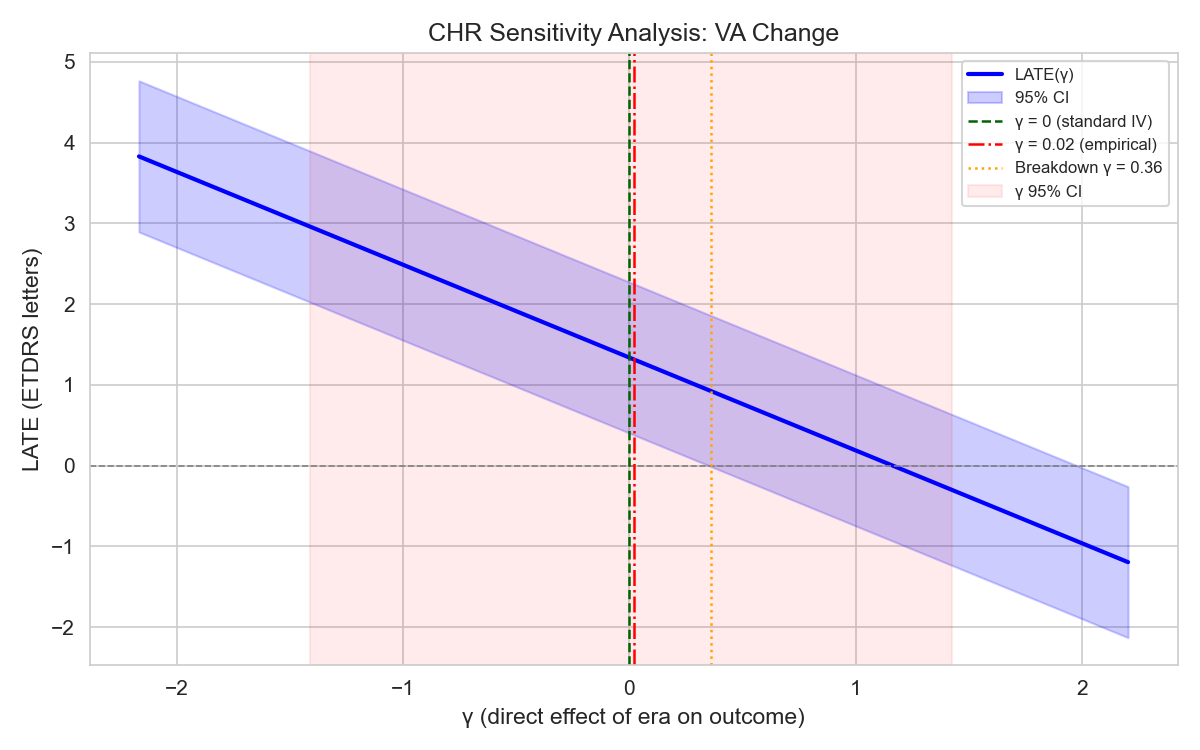
\includegraphics[width=0.85\textwidth]{figures/chr_sensitivity.png}
\caption{Exclusion-restriction sensitivity: LATE($\gamma$) for VA change with 95\% confidence band. The vertical dashed line marks $\gamma = 0$ (standard IV assumption); the solid line marks $\hat{\gamma}$. The breakdown value (0.36 letters) is the $\gamma$ at which the CI first includes zero.}
\label{fig:chr}
\end{figure}

\begin{figure}[H]
\centering
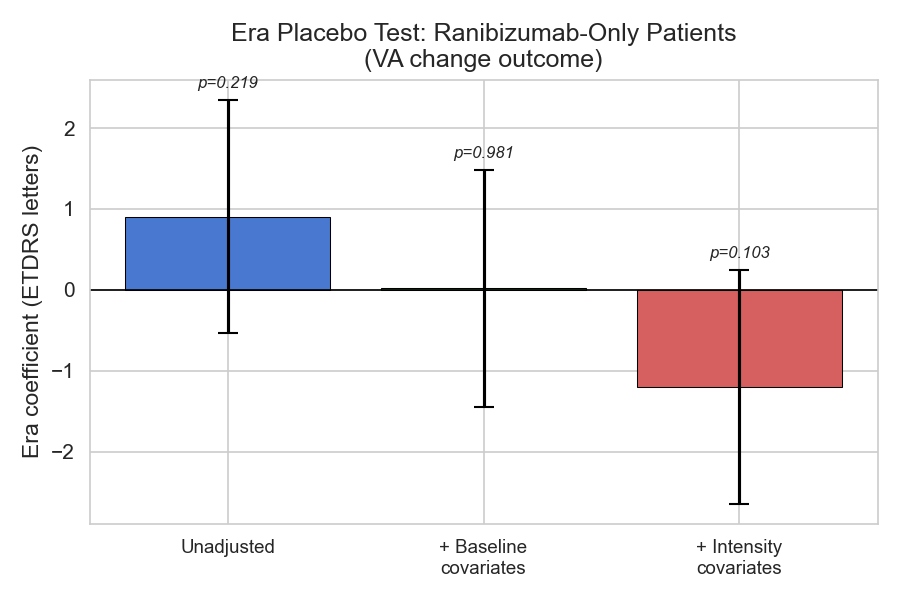
\includegraphics[width=0.7\textwidth]{figures/era_placebo.png}
\caption{Era coefficients among ranibizumab-only patients across specifications, illustrating differential instrument validity by outcome.}
\label{fig:placebo}
\end{figure}

The era placebo decomposition among ranibizumab-only patients shows the mechanism (Figure~\ref{fig:placebo}). The unadjusted era coefficient on VA change was $+0.91$ letters ($p = 0.22$); after baseline covariate adjustment it collapsed to $+0.02$ ($p = 0.98$). For VA~$\geq$~70, the era coefficient remained large and significant across all specifications: unadjusted $-0.138$ ($p < 0.001$), baseline-adjusted $-0.109$ ($p < 0.001$), intensity-conditioned $-0.073$ ($p < 0.001$). The concurrent shift from PRN to treat-and-extend dosing likely accounts for much of this residual era effect on the binary endpoint.

\begin{figure}[H]
\centering
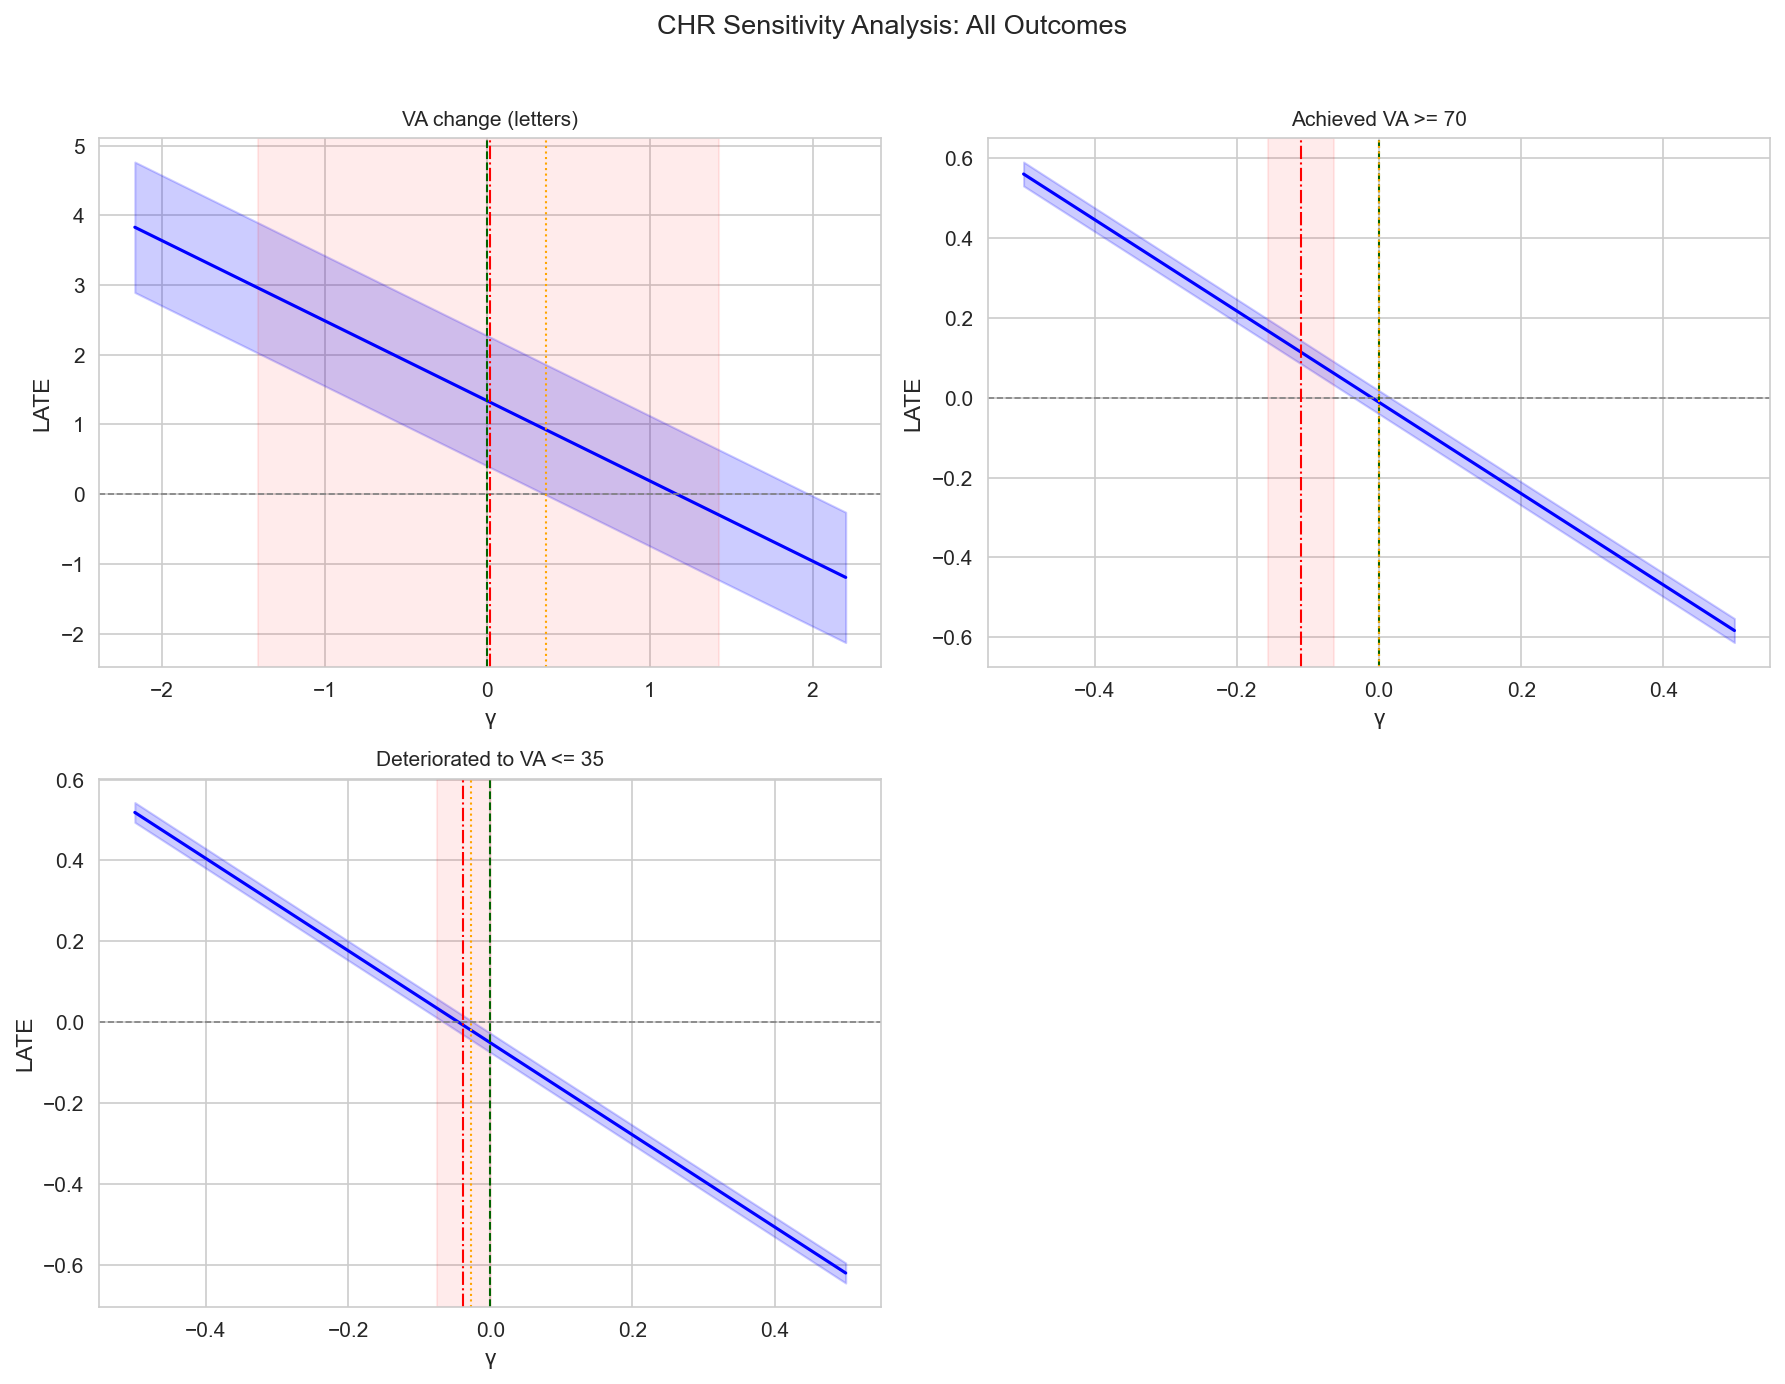
\includegraphics[width=0.85\textwidth]{figures/multi_outcome_sensitivity.png}
\caption{Multi-outcome sensitivity analysis: LATE($\gamma$) curves across all three endpoints, showing that binary outcomes are more fragile to exclusion-restriction violations.}
\label{fig:multi_outcome}
\end{figure}

Taken together, the sensitivity results and the instrument-independence failure point in the same direction: for continuous VA, the IV estimate is fragile --- a direct era effect below half a letter nullifies it. For the binary VA~$\geq$~70 endpoint, the IV assumption is already violated at the observed data.

\subsection{Heterogeneous treatment effects (Tier 3)}

Within the post-2013 restricted cohort ($n = 2{,}156$), raw outcome rates were nearly identical between arms (aflibercept 66.2\%, ranibizumab 66.0\%). The propensity model area under the receiver operating characteristic curve (AUC) was 0.555 --- treatment assignment was only weakly predicted by observed covariates (Figure~\ref{fig:cate_propensity}). While low AUC is favorable for overlap (reducing extrapolation), it does not rule out confounding from unobserved covariates.

\begin{figure}[H]
\centering
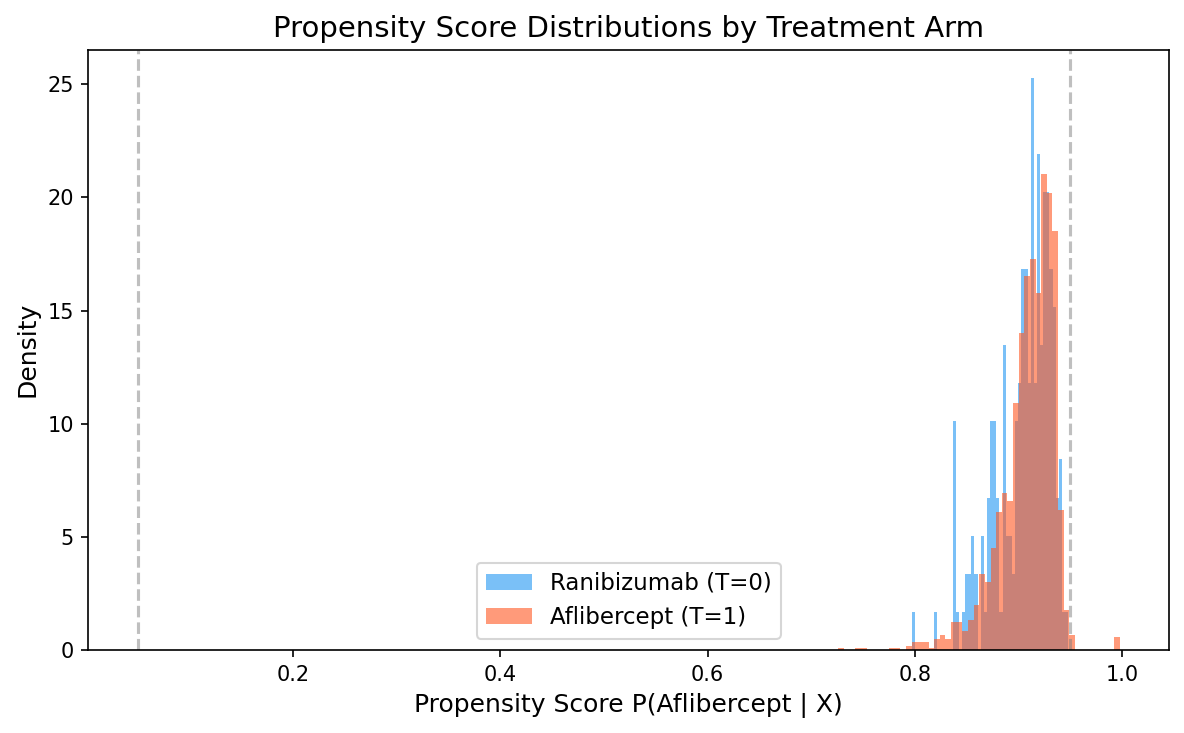
\includegraphics[width=0.7\textwidth]{figures/fig_propensity.png}
\caption{Post-2013 propensity score overlap (AUC = 0.555), showing near-random treatment assignment by observed covariates.}
\label{fig:cate_propensity}
\end{figure}

All five CATE estimators produced negative mean estimates: S-Learner ($-0.014$), T-Learner ($-0.041$), TARNet ($-0.011$), DragonNet ($-0.019$), X-Learner ($-0.019$). The AIPW ATE was $-0.022$ (95\% CI: $-0.046$ to $+0.002$). Figure~\ref{fig:cate_distributions} shows the overlaid CATE distributions. The X-Learner subgroup analysis identified induction-failure patients ($n = 177$) as the group with the largest estimated ranibizumab advantage (mean CATE: $-0.196$), but this variable is partly post-treatment and the subgroup carries high variance. For the dominant clinical subgroup (VA 50--69, age $>$ 80, $n = 690$), all methods estimated effects within two percentage points of zero (Figure~\ref{fig:cate_subgroups}).

\begin{figure}[H]
\centering

\includegraphics[width=0.85\textwidth]{figures/fig_cate_distributions.png}
\caption{CATE distributions from five estimators, all centered near or below zero.}
\label{fig:cate_distributions}
\end{figure}

\begin{figure}[H]
\centering
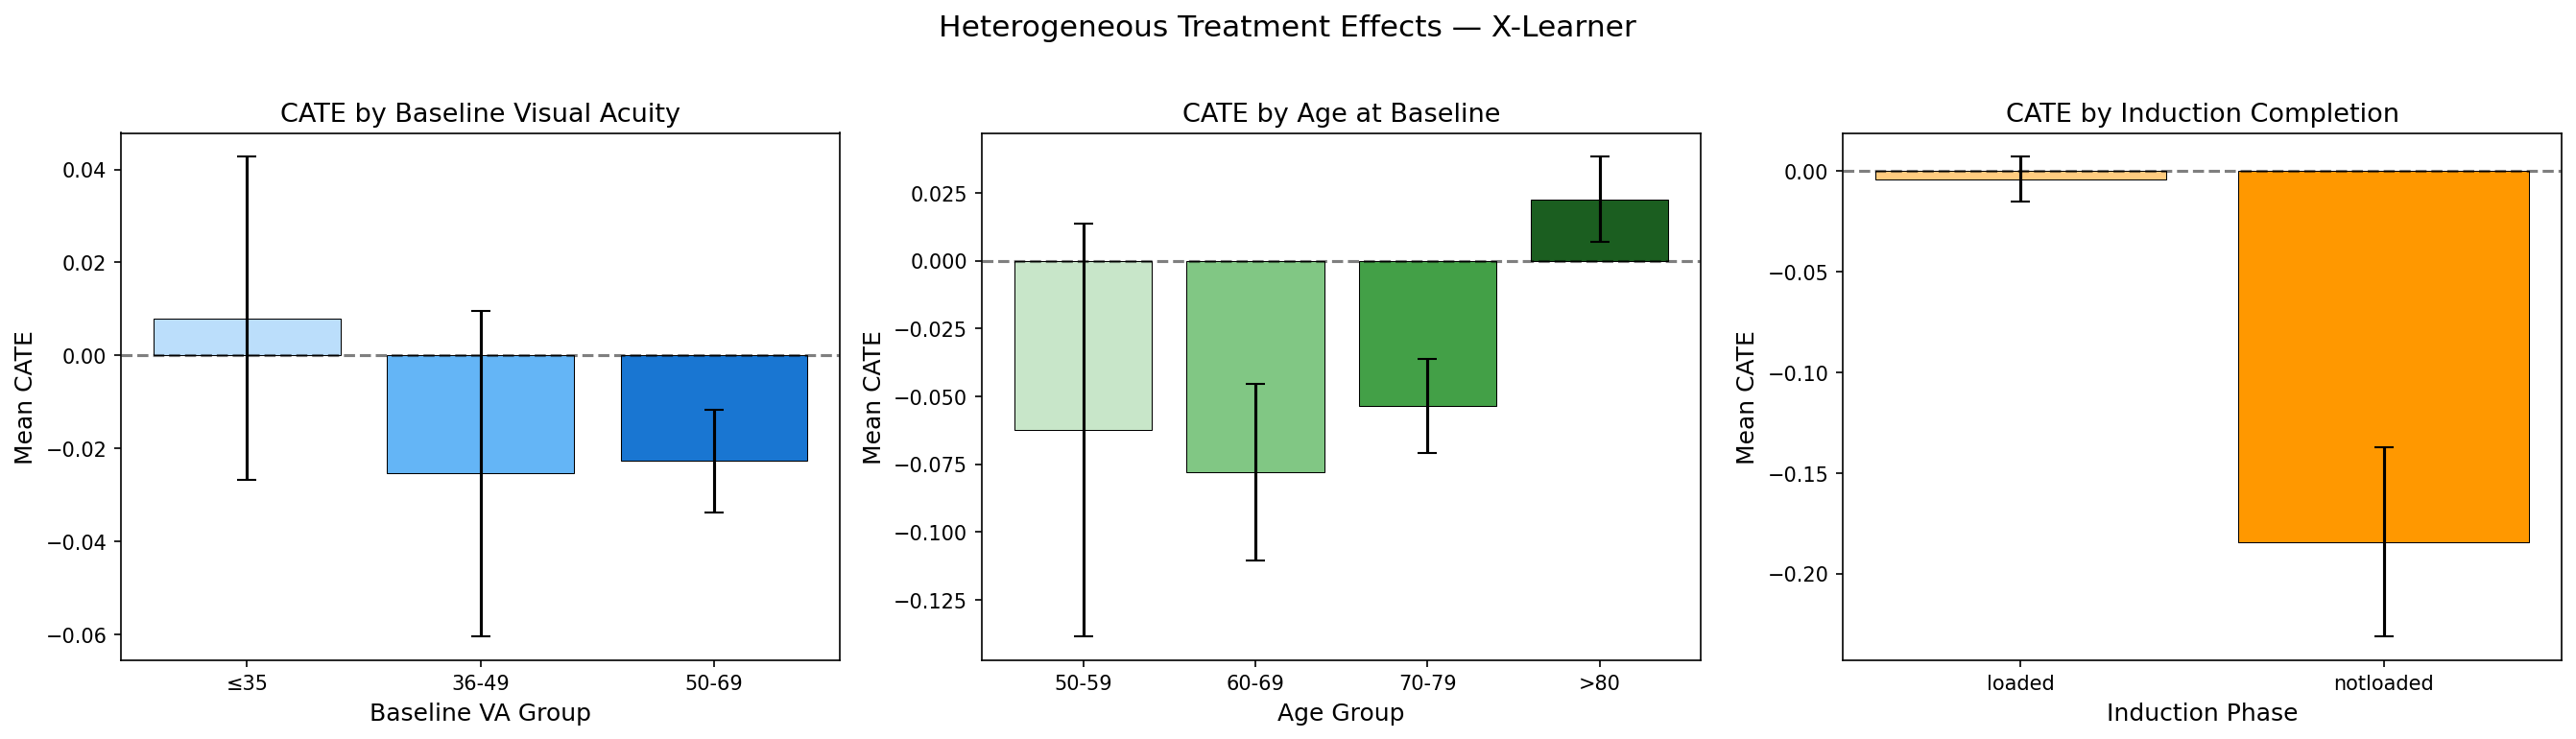
\includegraphics[width=0.85\textwidth]{figures/fig_cate_subgroups.png}
\caption{Subgroup CATE estimates by baseline VA, age, and induction completion.}
\label{fig:cate_subgroups}
\end{figure}

The unanimity across five distinct estimators --- with architectures ranging from gradient boosting to representation-learning networks --- is notable. No subgroup shows a reliable aflibercept advantage, and the largest signal (induction-failure patients) cannot support a causal claim given its post-treatment conditioning.

\subsection{Limitations}

Several design constraints bear on interpretation. Positivity is the most consequential: with 87\% of post-2013 patients on aflibercept, propensity scores cluster near the upper bound and the AIPW estimator relies heavily on outcome-model extrapolation, as the trimming analysis confirms. The binary era variable collapses the IV design from a fuzzy RDD to a standard IV, precluding bandwidth selection or local polynomial estimation. Differential follow-up --- up to 12 years for pre-2013 patients versus 6.3 for post-2013 --- introduces mechanical outcome differences; the sign reversal under follow-up restriction demonstrates this severity. De-identified age, available only as 10-year bands, limits covariate adjustment precision. The October 2013 introduction bundled drug access with protocol change: post-2013 ranibizumab patients may have remained on PRN while aflibercept patients received treat-and-extend, so the estimated contrast is between drug-protocol packages rather than drugs alone.

\section{Conclusion}

Once the drug-era confound is addressed, no identification strategy finds a clinically meaningful difference between aflibercept and ranibizumab on continuous VA change --- the outcome least susceptible to censoring artifacts. The apparent aflibercept advantage on binary endpoints traces to the concurrent protocol shift, not pharmacology. These observational results, obtained under substantially weaker assumptions than a randomized trial, nonetheless converge with trial-established equivalence \citep{heier2012}. Two caveats limit the strength of this conclusion: severe positivity violations force reliance on outcome-model extrapolation, and the drug-protocol confound cannot be fully separated with available data. Cost comparisons between the two agents vary by geography and formulary; bevacizumab, excluded from this dataset, remains the cheapest anti-VEGF option in most settings. Definitively resolving the drug-versus-protocol question would require either a pragmatic trial with standardized dosing or observational data that record drug assignment and protocol choice independently.

\bibliographystyle{plainnat}
\bibliography{references}

\end{document}
